%%% Copyright (C) 2017 David Beauchemin
%%%
%%% Ce fichier et tous les fichiers .tex ou .Rnw dont la racine est
%%% mentionnée dans les commandes \include ci-dessous font partie du
%%% projet «Actulab Co-operators 2017»
%%% https://github.com/davebulaval/Actulab_COOP
%%%
%%% Cette création est mise à disposition selon le contrat
%%% Attribution-Partage dans les mêmes conditions 4.0
%%% International de Creative Commons.
%%% http://creativecommons.org/licenses/by-sa/4.0/

\documentclass[11pt,french]{article}\usepackage[]{graphicx}\usepackage[]{color}
%% maxwidth is the original width if it is less than linewidth
%% otherwise use linewidth (to make sure the graphics do not exceed the margin)
\makeatletter
\def\maxwidth{ %
  \ifdim\Gin@nat@width>\linewidth
    \linewidth
  \else
    \Gin@nat@width
  \fi
}
\makeatother

\definecolor{fgcolor}{rgb}{0.345, 0.345, 0.345}
\newcommand{\hlnum}[1]{\textcolor[rgb]{0.686,0.059,0.569}{#1}}%
\newcommand{\hlstr}[1]{\textcolor[rgb]{0.192,0.494,0.8}{#1}}%
\newcommand{\hlcom}[1]{\textcolor[rgb]{0.678,0.584,0.686}{\textit{#1}}}%
\newcommand{\hlopt}[1]{\textcolor[rgb]{0,0,0}{#1}}%
\newcommand{\hlstd}[1]{\textcolor[rgb]{0.345,0.345,0.345}{#1}}%
\newcommand{\hlkwa}[1]{\textcolor[rgb]{0.161,0.373,0.58}{\textbf{#1}}}%
\newcommand{\hlkwb}[1]{\textcolor[rgb]{0.69,0.353,0.396}{#1}}%
\newcommand{\hlkwc}[1]{\textcolor[rgb]{0.333,0.667,0.333}{#1}}%
\newcommand{\hlkwd}[1]{\textcolor[rgb]{0.737,0.353,0.396}{\textbf{#1}}}%
\let\hlipl\hlkwb

\usepackage{framed}
\makeatletter
\newenvironment{kframe}{%
 \def\at@end@of@kframe{}%
 \ifinner\ifhmode%
  \def\at@end@of@kframe{\end{minipage}}%
  \begin{minipage}{\columnwidth}%
 \fi\fi%
 \def\FrameCommand##1{\hskip\@totalleftmargin \hskip-\fboxsep
 \colorbox{shadecolor}{##1}\hskip-\fboxsep
     % There is no \\@totalrightmargin, so:
     \hskip-\linewidth \hskip-\@totalleftmargin \hskip\columnwidth}%
 \MakeFramed {\advance\hsize-\width
   \@totalleftmargin\z@ \linewidth\hsize
   \@setminipage}}%
 {\par\unskip\endMakeFramed%
 \at@end@of@kframe}
\makeatother

\definecolor{shadecolor}{rgb}{.97, .97, .97}
\definecolor{messagecolor}{rgb}{0, 0, 0}
\definecolor{warningcolor}{rgb}{1, 0, 1}
\definecolor{errorcolor}{rgb}{1, 0, 0}
\newenvironment{knitrout}{}{} % an empty environment to be redefined in TeX

\usepackage{alltt}
  \usepackage{babel} %%french
  \usepackage{amsmath,amsfonts,amssymb} %%maths
  \usepackage[utf8]{inputenc}   % LaTeX
  \usepackage[T1]{fontenc}      % LaTeX
  \usepackage[dvipsnames,table,xcdraw]{xcolor}
  
  %% image
  \usepackage{graphicx}
  	\graphicspath{{./fig/}} %fig path
  %%lien hypertex
  \usepackage[colorlinks, allcolors=Blue]{hyperref} 
  %% package pour modifier les chapitres #2
  \usepackage{titlesec}
  %% for number separation
  \usepackage[autolanguage]{numprint}
  \setcounter{tocdepth}{4}
  \setcounter{secnumdepth}{4}

%% for licence
  \usepackage{tabularx}
  \usepackage{multirow}
  %% no indent
  \setlength{\parindent}{0pt}
  \frenchbsetup{StandardItemLabels=true} % pour obtenir des puces par défaut dans les listes à puces A.B.
  %% for moreInfo 
  \usepackage{fontawesome} %%also cool logo
  \usepackage[framemethod=TikZ]{mdframed}
  
  % Commande pour licence voir github
  \newcommand{\viewsource}[1]{%
  \href{#1}{%
      Voir sur GitHub \raisebox{-1pt}{\footnotesize\faGithub}}}
   \newcommand{\ghurl}{https://github.com/davebulaval/Actulab_COOP}
  
  % Creation of environment to add additional informations
  % Provided by Samuel Cabral Cruz
\mdfsetup{
	linewidth=2pt,
	nobreak=true,
	backgroundcolor=Blue!10,
	roundcorner=10pt}	
\newenvironment{moreInfo}[1]
	{\begin{mdframed}
	\textcolor{darkgray}{\huge \raisebox{-3.5pt}{\faInfo} 
	\hspace{0.5cm} \large\bfseries #1}\\[5pt]
	\normalsize
	\makebox[0.1\textwidth][l]{}	
	\begin{minipage}{10cm}}
	{	\end{minipage}
	\end{mdframed}}

%% Changement font TOC
\usepackage{tocloft}
\renewcommand\cftpartfont{\LARGE\bfseries}
\renewcommand\cftpartpagefont{\LARGE\bfseries}

%% meta donnée document
\title{Résolution de problématique de \\ Co-Operators \\ \bigskip Où sont les clients que nous ciblons ?}
\author{\textbf{Présenter par \\ David Beauchemin}}
\date{\today}
 
%header
\usepackage{fancyhdr}
\pagestyle{fancy}
\fancyhf{}
\lhead{Où sont les clients que nous ciblons ?}
\rhead{Co-operators}
\IfFileExists{upquote.sty}{\usepackage{upquote}}{}
\begin{document}


\makeatletter
  \begin{titlepage}
  \centering
      {\fontsize{52}{52} \textbf{\textsc{Actulab}}}\\
    \vspace{2cm}
    \vspace{2cm}
    \vspace{2cm}
      {\fontsize{20}{20}\textbf{\@title}} \\
    \vfill
       {\Huge \@author} \\
    \vspace{8cm}
    \vfill
  \end{titlepage}
\makeatother

%%%%license %%%%%
\small
{\copyright} {\the\year} David Beauchemin \\

\vspace{\baselineskip}


\includegraphics[height=7mm,keepaspectratio=true]{by-sa}\\%
Cette création est mise à disposition selon le contrat
\href{http://creativecommons.org/licenses/by-sa/4.0/deed.fr}{%
  Attribution-Partage dans les mêmes conditions 4.0 International} de
Creative Commons. En vertu de ce contrat, vous êtes libre de:
\begin{itemize}
\item \textbf{partager} --- reproduire, distribuer et communiquer
  l'{\oe}uvre;
\item \textbf{remixer} --- adapter l'{\oe}uvre;
\item utiliser cette {\oe}uvre à des fins commerciales.
\end{itemize}
Selon les conditions suivantes:

\begin{tabularx}{\linewidth}{@{}lX@{}}
  \raisebox{-9mm}[0mm][13mm]{%
    
\includegraphics[height=11mm,keepaspectratio=true]{by}} &
  \textbf{Attribution} --- Vous devez créditer l'{\oe}uvre, intégrer
  un lien vers le contrat et indiquer si des modifications ont été
  effectuées à l'{\oe}uvre. Vous devez indiquer ces informations par
  tous les moyens possibles, mais vous ne pouvez suggérer que
  l'offrant vous soutient ou soutient la façon dont vous avez utilisé
  son {\oe}uvre. \\
  \raisebox{-9mm}{
\includegraphics[height=11mm,keepaspectratio=true]{sa}}
  & \textbf{Partage dans les mêmes conditions} --- Dans le cas où vous
  modifiez, transformez ou créez à partir du matériel composant
  l'{\oe}uvre originale, vous devez diffuser l'{\oe}uvre modifiée dans
  les mêmes conditions, c'est-à-dire avec le même contrat avec lequel
  l'{\oe}uvre originale a été diffusée.
\end{tabularx}

\bigskip
  \textbf{Code source} \\
  \viewsource{\ghurl}
\pagebreak

\tableofcontents

\clearpage

%%%%%% SOMMAIRE %%%%%%%%
\part{Rapport sommaire}

\section{Détails techniques sommaires}

\subsection*{Analyse du mandat}

Déterminer la distribution d'une ou plusieurs variables sur un territoire. Prédire la distribution des personas sur un territoire à l'aide de la distribution des variables.

\subsection*{Collecte des données}

Voici la liste des différents rapports et données ayant été utilisés lors de la réalisation du rapport :

\begin{itemize}
\item Données libres du recensement canadien de \href{http://www12.statcan.gc.ca/census-recensement/2016/dp-pd/prof/details/download-telecharger/comp/page_dl-tc.cfm?Lang=F}{2016} 
\item Listes des études utilisées pour les hypothèses :
     \begin{itemize}
     \item Bulletin d'information statistique du ministère de la Famille du Québec : \href{https://www.mfa.gouv.qc.ca/fr/Famille/chiffres-famille-quebec/bulletin_quelle_famille/Pages/aut2013_no1_tab4.aspx}{Quelle famille ?};
     \item Enquête nationale auprès des ménages \href{http://www12.statcan.gc.ca/nhs-enm/2011/dp-pd/dt-td/Rp-fra.cfm?TABID=2&LANG=F&A=R&APATH=3&DETAIL=0&DIM=0&FL=A&FREE=0&GC=24&GL=-1&GID=1118301&GK=1&GRP=1&O=D&PID=106042&PRID=0&PTYPE=105277&S=0&SHOWALL=0&SUB=0&Temporal=2013&THEME=96&VID=0&VNAMEE=&VNAMEF=&D1=2&D2=0&D3=0&D4=0&D5=0&D6=0}{2011};
     \item Statistiques de l'enseignement supérieur \href{http://www.education.gouv.qc.ca/fileadmin/administration/librairies/documents/Ministere/acces_info/Statistiques/Statistiques_ES/Statistiques_enseignement_superieur_2013.pdf}{2013}.
     \end{itemize}
\item Polygones des régions de tri d'acheminement \href{http://www12.statcan.gc.ca/census-recensement/2011/geo/bound-limit/bound-limit-2016-fra.cfm}{national}
\item Listes des régions de tri \href{https://fr.wikipedia.org/wiki/Liste_des_codes_postaux_canadiens_débutant_par_J}{d'acheminement}
\end{itemize}

\section{Hypothèse utilisée}

Hypothèses utilisées pour le projet :
\begin{enumerate}
\item Indépendance entre les variables
\item Distribution uniforme sur les intervalles d'âges
\item Distribution uniforme des travailleurs (provincial)
\item Distribution uniforme des étudiants (provincial)
\item Distribution uniforme des colocataires (provincial)
\item Retraite à 65 ans
\end{enumerate}

\section{Application \emph{Shiny}}

Afin de visualiser la distribution des personas et de permettre une flexibilité d'analyse future, une application \href{https://www.rstudio.com/products/shiny/}{\emph{Shiny}} à été développée. L'application en soi correspond aux résultats de la modélisation et constitue l'ensemble du projet. Cette \href{https://davebulaval.shinyapps.io/personnasIdentificateur/}{application} permet de:
\begin{itemize}
\item sélectionner les différentes variables à modéliser;
\item de modéliser visuellement la densité de la distribution;
\item d'afficher les territoires observés;
\item d'afficher, par région de tri d'acheminement, la population totale et la prédiction du nombre de personas identifier dans cette région.
\end{itemize}

\begin{moreInfo}{\color{Gray}\emph{Utilisation}
     \color{black}}
Pour utiliser l'application, il suffit d'accéder à la page web et de sélectionner les variables désirées. Pour afficher les informations de la région de tri d'acheminement, il suffit de glisser le curseur sur celle-ci.
     \newline
     Le délai d'exécution peut parfois prendre quelques secondes. 
\end{moreInfo}

\section{Résultat sommaire}

Les distributions du persona 1 et du persona 5 peuvent être ajustées selon des lois Normales. Par contre, pour les trois autres personas, le modèle ne permet pas d'ajuster à une loi de distribution connue. On peut consulter les prédictions des personas plus loin dans le rapport.

\section{Code source}

Il est possible de consulter l'ensemble du code source et les données utilisées pour le projet à partir de la \href{https://davebulaval.github.io/Actulab_COOP/}{page web} du dépôt \href{https://github.com/davebulaval/Actulab_COOP}{\emph{GitHub}}.

\section{Auteur}
\href{mailto:david.beauchemin.5@ulaval.ca}{David Beauchemin}, étudiant en actuariat à l'Université Laval.


\newpage
%%%%%% Content %%%%%%%%
\part{Rapport détaillé}

\section{Détails de la problématique}

Étant une coopérative d'assurance, Co-operators utilise un réseau de distribution à l'aide de différentes agences dispersées à l'échelle nationale. Celles-ci offrent un ensemble  de produits d'assurances vie et d'assurances dommages.
\newline

Afin d'offrir un support amélioré aux différentes agences d'assurances de Co-operators, la définition de certaines caractéristiques de profil type est extraite des données clients.  Afin de déterminer la nature de la modélisation des variables, l’utilisation des données libres est utilisée pour construire et représenter la distribution.

\section{Détails techniques}

\subsection{Mandat}

Le mandat de cette problématique Actulab correspond à déterminer la distribution des différentes variables observées des personas en plus de toutes autres variables jugées pertinentes. Cette distribution doit pouvoir être représentée sur un territoire avec une échelle de région de tri d'acheminement (RTA).
\newline

Prédire la distribution des personas sur un territoire avec une échelle de RTA à l'aide de la distribution des variables des personas. La modélisation des personas et de leurs variables doit provenir de données en source libre et gratuite. 
\newline

La modélisation des personas permettra d'offrir une personnalisation des produits, une meilleure approche client ainsi que de mieux cibler le style de communication entre Co-operators et les personas.

Le projet sera remis à Co-operators dans le cadre du projet Actulab 2017.

\subsection{Collecte des données}

Depuis l'essor du \emph{Big Data} et du \emph{deep learning}, de nombreuses bases de données sont devenues disponibles gratuitement en ligne. Ce mouvement de \emph{démocratisation} des données a aussi été incorporé auprès de nombreuses instances gouvernementales. À cet effet, Statistique Canada, offre l'ensemble des jeux de données des recensements depuis 1991. De plus, de nombreux rapports et jeux de données provinciales sont aussi disponibles. Cet accès à un nombre important de données a permis de résoudre la problématique abordée.
\newline

Parmi les données utilisées ,on retrouve le recensement canadien \href{http://www12.statcan.gc.ca/census-recensement/2016/dp-pd/prof/details/download-telecharger/comp/page_dl-tc.cfm?Lang=F}{2016}.  La segmentation des données a déjà été effectuée en RTA par statistique Canada. Cette base de données contient de nombreuses variables essentielles à l’analyse. On retrouve, la population par RTA, le nombre de femme et d’homme par RTA, le nombre de personnes par tranches de salaire et beaucoup d’autres encore.
\newline

Il faut aussi noter que pour des fins de simplification, seulement la province du Québec a été étudiée. De plus, une liste réduite de villes a été sélectionnée pour représenter cartographiquement les variables sur le territoire. Afin de modéliser la distribution des variables non segmentées par RTA, différentes hypothèses ont été retenues. Celles-ci seront discutées plus loin. 
\newline

Pour soutenir la crédibilité des hypothèses, des publications et des études de différents départements nationaux ou provinciaux ont été étudiées pour en dégager les grandes tendances. 
\newline

Tout d'abord, afin de mieux représenter la réalité familiale dans la province du Québec le bulletin d'information statistique du ministère de la Famille a été utilisé. Le bulletin, \href{https://www.mfa.gouv.qc.ca/fr/Famille/chiffres-famille-quebec/bulletin_quelle_famille/Pages/aut2013_no1_tab4.aspx}{\emph{Quelle famille ?}}, a permis d'établir le comportement général de la population à l'égard de la colocation. On remarque une plus grande proportion de colocation pour les personnes de plus de 70 ans. Ces différentes proportions de la population habitant en colocationont été utilisées pour déterminer la probabilité d'un résident d'habiter en colocation. Il est à noter que ces données ne sont pas segmentées par RTA.
\newline

De plus, l'enquête nationale auprès des ménages de \href{http://www12.statcan.gc.ca/nhs-enm/2011/dp-pd/dt-td/Rp-fra.cfm?TABID=2&LANG=F&A=R&APATH=3&DETAIL=0&DIM=0&FL=A&FREE=0&GC=24&GL=-1&GID=1118301&GK=1&GRP=1&O=D&PID=106042&PRID=0&PTYPE=105277&S=0&SHOWALL=0&SUB=0&Temporal=2013&THEME=96&VID=0&VNAMEE=&VNAMEF=&D1=2&D2=0&D3=0&D4=0&D5=0&D6=0}{2011} a permis d'établir les hypothèses sur les professions des Québécois. Ces différentes données sur l'emploi, on permit d'établir la probabilité d'un résident d'occuper une profession quelconque Le jeu de donnée ne contient pas le nombre d'étudiants étant donné que les étudiants ne font pas partie de la population active. Afin de déterminer la proportion de la population québécoise étudiante, le rapport des statistiques de l'enseignement supérieur de \href{http://www.education.gouv.qc.ca/fileadmin/administration/librairies/documents/Ministere/acces_info/Statistiques/Statistiques_ES/Statistiques_enseignement_superieur_2013.pdf}{2013} a été utilisé. Celui-ci a permis d'établir la proportion d'étudiants dans chacun des différents établissements collégiaux et universitaires. Autrement dit, la région métropolitaine de résidence. De plus, il a permis d'établir la probabilité d'être un étudiant. Il est à noter que ces données ne sont pas segmentées par RTA.
\newline

Finalement, afin de représenter cartographiquement les prédictions et les variables, les données sur les polygones des régions de tri d'acheminement \href{http://www12.statcan.gc.ca/census-recensement/2011/geo/bound-limit/bound-limit-2016-fra.cfm}{national} ont été utilisées. Il s'agit de la correspondance cartographique des RTA sous forme d'un polynôme à multiple côté. Ainsi, il a été possible de représenter dans l'application la distribution. Afin de déterminer les codes postaux des villes étudiées, la liste des régions de tri \href{https://fr.wikipedia.org/wiki/Liste_des_codes_postaux_canadiens_débutant_par_J}{d'acheminement} a été utilisée. Il s'agit essentiellement des codes postaux par ville ou arrondissement.


\subsection{Traitement des données}

Avant de débuter la manipulation des données, l'analyse des caractéristiques des personas a permis de ressortir les différents besoins en données ainsi que les possibles manipulations à effectuer. 

\subsubsection{Caractéristiques des personas}
On note les caractéristiques suivantes pour les différents profils types :

\subsubsection*{Persona 1}
\label{per1}
\begin{itemize}
\item[Âge :] entre 16 et 26 ans - (Génération \emph{millenials});
\item[Salaire annuel :] \numprint{20000} \$
\item[Occupation :] Étudiant
\end{itemize}

\subsubsection*{Persona 2}
\label{per2}
\begin{itemize}
\item[Âge :] entre 32 et 39 ans - (fin de la génération \emph{x} et début de la génération \emph{millenials});
\item[Occupation :] Comptable
\item[Salaire annuel :] \numprint{51000} \$
\end{itemize}

\subsubsection*{Persona 3}
\label{per3}
\begin{itemize}
\item[Âge :] entre 40 et 52 ans - (Génération \emph{x});
\item[Occupation :] Travailleur autonome - propriétaire d'une PME
\item[Salaire annuel :] \numprint{105000} \$
\end{itemize}

\subsubsection*{Persona 4}
\label{per4}
\begin{itemize}
\item[Âge :] entre 53 et 65 ans - (Génération \emph{baby-boom});
\item[Occupation :] Enseignante
\item[Salaire annuel :] \numprint{50000} \$
\end{itemize}

\subsubsection*{Persona 5}
\label{per5}
\begin{itemize}
\item[Âge :] entre 66 et 76 ans - (Génération \emph{baby-boom});
\item[Occupation :] Retraité
\item[Salaire annuel :] \numprint{43000} \$
\end{itemize}
\bigskip

Pour l'ensemble des personas,  les caractéristique d'âge, d’état civil et de type d'occupation peuvent facilement être extraites du recensement. Par contre, pour les autres variables telles que  des hypothèses et de la simplification ont été nécessaires pour obtenir l'information.
\newline

En ayant les différentes caractéristiques nécessaires à l’analyse, la segmentation des données d’âges, de salaire, de profession et autres a été effectuée. Afin de faciliter l’utilisation et de diminuer la charge sur l’application, les données découpées à partir des différents jeux de données ont été enregistrées dans un nouveau jeu de donnée.

\section{Objectif}

L'objectif de ce projet est de répondre aux mandats de Co-operators, soit d'offrir une analyse prédictive de la distribution des personas et d'offrir une application permettant d'observer cette distribution sur le territoire.

\section{Outils utilisés}

Les différents outils numériques utilisés lors de la résolution de cette problématique sont l'utilisation de statistique R. Ayant une solide formation informatique avec R, l'utilisation de ce langage parait plutôt évidente. Par contre, on note différents avantages notables de R par rapport aux différentes alternatives telles qu’ Excel/VBA ou Python. Tout d'abord, la possibilité de créer une application \emph{Shiny} est l'une des principales motivations qui ont justifié l'utilisation de R. De plus, la grande communauté R et la quantité importante de \emph{package} à aussi permis de traiter les fichiers de polygone cartographique et l'affichage d'une carte dynamique. Ces deux avantages ont dans leurs ensembles été déterminants dans la décision d'utiliser R.
\bigskip

\begin{moreInfo}{\color{Gray}À propos de \emph{Shiny}
     \color{black}}
     Une application \href{https://shiny.rstudio.com}{\emph{Shiny}} correspond à une application écrite en R qui utilise un serveur pour effectuer les calculs. Cette application sera donc disponible sur une page web. L'utilisation sous certaines conditions est gratuite via  \href{https://www.shinyapps.io}{\emph{Shinyapps}}.
\end{moreInfo}

\section{Méthodologie}

Le principal enjeu de ce projet est la validité de la prédiction de la distribution des caractéristiques. Afin de bien représenter celles-ci sur le territoire, certaines hypothèses ont été nécessaires afin de simplifier le modèle et de permettre la réalisation du mandat.
\newline

\subsection{Indépendance des variables}

Tout d'abord, une hypothèse essentielle est l'indépendance entre les variables. Il s'agit d'une hypothèse courante en modélisation et celle-ci permet de simplifier le modèle. Grâce à cette hypothèse, l'ajout de variable dans le modèle a été beaucoup plus facile à réaliser. En effet, pour prédire le nombre de personas correspondant à une série de caractéristiques, on applique le concept suivant :
\begin{align*}
f_{\mathbb{X}}(x) &= f_{X_1}(x_1) \times ... \times f_{X_n}(x_n)
\end{align*}
Où $\mathbb{X}$ est un vecteur de n variables et $X_i$ est la variable caractéristique i.
\newline

Ainsi, si on recherche le nombre d'étudiants de 16 à 26 ans habitant en colocation, on utilise 
\begin{align*}
f_{\mathbb{X}}(x) &= f_{X_{\text{Occupation}}}(x) \times f_{X_{\text{Âge}}}(x) \times f_{X_{\text{Colocation}}}(x)
\end{align*}
Il devient ainsi beaucoup plus simple de modéliser la fonction conjointe des différentes variables. 
\newline


Étant donné la segmentation originale du recensement, il est possible de valider l'hypothèse. En effet, à l'aide du test de khi-deux, il est possible de vérifier l'hypothèse entre les variables. Par exemple, si on teste avec la population d'homme âgé entre 16 et 26 ans on obtient la \emph{p-value} suivante :
\begin{knitrout}
\definecolor{shadecolor}{rgb}{0.969, 0.969, 0.969}\color{fgcolor}\begin{kframe}
\begin{alltt}
\hlstd{chisqTest}\hlopt{$}\hlstd{p.value}
\end{alltt}
\begin{verbatim}
## [1] 0.4189084
\end{verbatim}
\end{kframe}
\end{knitrout}
Autrement dit, le test est non significatif et ne permet pas de rejeter l'hypothèse d'indépendance entre les variables. 

\subsection{Distribution uniforme sur les intervalles d'âges}

De plus, une seconde hypothèse importante est la distribution sur les intervalles d'âges. Il a été supposé que, sur l'intervalle d'âge de $x$ ans à $x + c$ ans, la répartition est distribuée uniformément. Autrement dit, la probabilité d'avoir $x$ ans est la même que d'avoir $x + c$ ans. Cette hypothèse permet d'effectuer une interpolation sur la segmentation du recensement. Les intervalles d’âges n’étant pas ceux recherchés, il a ainsi été possible de construire les intervalles d'âges des personas. Cette hypothèse n'a pas été mathématiquement testée, mais en considérant une certaine constante dans le taux de natalité, hormis le baby-boom d'après-guerre, il est convenable de dire que la distribution est uniforme.

\subsection{Distribution uniforme des travailleurs}

Les trois prochaines hypothèses ont été les plus difficiles à établir et à valider. Elles sont importantes dans l'analyse. Ayant peu de données segmentées sur les travailleurs, il a été difficile de bien capter l'information. En effet, depuis la simplification du formulaire de recensement, le domaine d'occupation n'est pas inclus dans le recensement de 2011 et 2016. Par contre, l'enquête nationale auprès des ménages contient l'information à l'échelle provinciale. Étant donner que l'information a été segmentée en onze secteurs d'occupations, l'hypothèse suivante semblait adéquate. Soit que la distribution des 11 catégories d'occupation est uniformément distribuée dans la province. Autrement dit, la probabilité de retrouver un gestionnaire dans la RTA X1X est la même que dans la RTA X2X. Cela a ainsi permis de capter une partie de l'information sur l'occupation professionnelle des personas. 

\subsection{Distribution uniforme des étudiants}

Toujours dans l'occupation des personas, la distribution de la caractéristique étudiante n'est pas incluse dans le recensement. En effet, les étudiants ne sont pas compris dans la population active, il devient donc difficile de segmenter l'information jusqu'à la RTA. Pour trouver la proportion des étudiants pour l'ensemble du Québec, la contribution du rapport sur les statistiques de l'enseignement supérieur fut nécessaire. Celui-ci a permis d'établir le nombre d'étudiants qui fréquentent un établissement d'enseignement supérieur. En consultant les chiffres, on constate qu'environ 50 \% de la population étudiante fréquente un établissement Collégiale de Montréal et de 60 \% pour un établissement universitaire. Il devient donc difficile de déterminer la distribution des étudiants en périphérie des établissements scolaires. En supposant que l'étalement urbain autour de cet établissement est exponentiellement décroissant selon la facilité d'accès via le transport en commun et le réseau routier normal. On peut supposer une certaine distribution uniforme des étudiants dans les régions avoisinantes. Il a été ainsi conclu que l'hypothèse de distribution uniforme des étudiants sur le territoire est plausible et sera utilisée pour le projet. L'analyse d'une piste de solution sur cette variable est abordée plus loin.

\subsection{Distribution uniforme des colocataires}

Pour cette dernière hypothèse de distribution, pour les mêmes raisons de disponibilité de l'information ainsi que la difficulté de segmentation. Il était difficile de bien modéliser la variable. Toutefois, à l'aide du bulletin du ministère de la Famille, le comportement des Québécois en matière de colocation a été étudié. L'étude fait état d'une variation plus ou moins grande selon l'intervalle d'âge et la région. Étant donné que les intervalles d'âge sont relativement large la distribution uniforme sur la colocation semblait approprié et adéquate. Cette hypothèse a donc été retenue, ce qui permet de simplifier grandement le modèle. 

\subsection{Retraite à 65 ans}

Afin de simplifier le modèle, l'hypothèse de retraite à l'âge unique de 65 ans a été retenue. En effet, il était difficile de bien modéliser la retraite progressive, la retraite anticipée, la retraite \emph{normale} et la retraite prolongée. Le principal facteur de cette hypothèse a été le facteur temps dans la réalisation du projet. À partir des données disponibles sur la retraite de Retraite Québec, la modélisation de cette variable aurait été plus complétée.
\newline

Pour conclure, les différentes hypothèses retenues ont permis de construire le modèle de façon simple et cohérente à partir des informations disponibles.

\section{Avantage-Inconvénient}

Tout modèle n'étant pas parfait, des avantages et inconvénients sont à prendre en considération pour chacun d'eux. Le modèle présenter ici ne faisant pas exception à cette règle, celui-ci entraine de nombreux avantages et de nombreux inconvénients. 
\newline

Tout d'abord, la simplicité de l'hypothèse d'indépendance entre les variables permet de facilement capter une bonne partie de l'information. Elle permet de modéliser les variables avec simplicité. Cette simplicité permet aussi d'ajouter de nombreuses variables aux modèles, il devient ainsi possible de rajouter des variables telles que le bilinguisme, le nombre d'enfants et le type de résidence. Cet avantage est la principale motivation ayant justifié l'hypothèse d'indépendance du modèle.
\newline

De plus, en supposant la distribution uniforme de certaines variables, il fut possible de modéliser des variables plus difficiles à modéliser. Par exemple, la colocation aurait été beaucoup plus difficile à modéliser dans un modèle sans distribution uniforme. 
\newline

La simplicité globale du modèle a aussi permis la création d'une application web, ce qui permet à toutes les agences du réseau de consulter en temps réel le modèle. Il ne devient donc plus nécessaire de faire affaire avec un intermédiaire en centre d'expertise. Situation très intéressante dans un contexte d'affaires.
\newline

Par contre, l'indépendance entre les variables entraine une perte d'information lorsque le nombre de variables à modéliser devient important. En effet, il devient difficile de bien \emph{supporter} l'hypothèse d'indépendance entre toutes les variables. Cette simplicité de modèle est intéressante pour les variables déjà présentes dans les données du recensement. Par contre, lorsqu'il s'agit de représenter des variables n'ayant pas été segmentées par RTA, la qualité du modèle peut ne pas être toujours très satisfaisante.
\newline

De plus, l'utilisation de l'application étant intéressante, son interprétation peut être trompeuse et induire en erreur des décisions d'affaires des différentes agences.

Pour conclure, dans son ensemble le modèle présenter représente bien la réalité de la distribution des personas. L'amélioration du modèle via les différentes pistes de solution discuter plus loin pourrait amener le modèle à mieux prédire la distribution.
 
\section{Résultats}

Pour des fins de simplification seulement la région de Laval sera étudiée pour l'analyse des résultats. Cette analyse sera divisée par persona, afin de bien comprendre leur distribution.
Tout d'abord, si on effectue une analyse pour l'ensemble de la province, on remarque les tendances macro-provinciales suivantes : 
\bigskip

\begin{itemize}
\item Moyenne de population par RTA : \numprint{19848}
\item Maximum de population par RTA : \numprint{139125}
\item Minimum de population par RTA : \numprint{560}
\end{itemize}


\subsection{Jacob}
Le persona de Jacob possède les caractéristiques suivantes : 
\begin{itemize}
\item 20 ans;
\item\numprint{20000} \$;
\item étudiant.
\end{itemize}
La fonction de prédiction correspond à

\begin{align*}
f_{\mathbb{X}}(x) &= f_{X_{\text{Occupation}}}(\text{Étudiant}) \times f_{X_{\text{Âge}}}(\text{16-26}) \times f_{X_{\text{salaire}}}(\text{\numprint{20000} - \numprint{30000}})
\end{align*}

Ce qui nous permet de trouver le tableau de valeur suivant :
\begin{knitrout}
\definecolor{shadecolor}{rgb}{0.969, 0.969, 0.969}\color{fgcolor}\begin{kframe}
\begin{verbatim}
## # A tibble: 19 x 5
##       X1 Prediction `Pop homme 16_26` `Pop etudiante` Salaire
##    <chr>      <int>             <int>           <dbl>   <int>
##  1   H7A         12              1477      0.06286751    2660
##  2   H7B          1               191      0.06286751     370
##  3   H7C          4               533      0.06286751    1165
##  4   H7E         15              1891      0.06286751    3330
##  5   H7G         13              1373      0.06286751    3180
##  6   H7H          7               964      0.06286751    1620
##  7   H7J          1               125      0.06286751     325
##  8   H7K         13              1686      0.06286751    2735
##  9   H7L         16              2518      0.06286751    3735
## 10   H7M         18              1978      0.06286751    4060
## 11   H7N         32              3027      0.06286751    7065
## 12   H7P         20              2388      0.06286751    4635
## 13   H7R         16              1962      0.06286751    3880
## 14   H7S          6               545      0.06286751    1230
## 15   H7T         15              1582      0.06286751    3750
## 16   H7V         16              1303      0.06286751    4440
## 17   H7W         32              2630      0.06286751    8130
## 18   H7X         14              1823      0.06286751    3200
## 19   H7Y          3               615      0.06286751     875
## [1] 13
\end{verbatim}
\end{kframe}
\end{knitrout}
On remarque que la moyenne correspond à 13 pour l'ensemble du territoire de l'ile de Laval. Le résultat est cohérent avec les données initiales du recensement. En effet,
selon les données de Statistique Canada, il y a en moyenne 1506 hommes âgés de 16 et 26 ans par région de tri d'acheminement. De plus, la proportion d'étudiant est de $6.286751 \%$ pour l'ensemble des RTA. Ce qui donne en moyenne 95 hommes âgés de 16 et 26 ans et qui sont étudiant par RTA. En ajoutant cette dernière variable de salaire, on réduit encore plus notre échantillon de la population qui correspond aux variables. \newline

On note que l'hypothèse d'indépendance entre la variable population âgée de 16 et 26 ans et la variable occupation étudiante est difficile à ne pas remettre en doute. Toutefois, tel que mentionné plus haut, celle-ci permet de simplifier le modèle. Il est possible de consulter la distribution des \emph{Jacob} à l'aide de l'application.

\subsubsection*{Analyse des graphiques de distribution}

On présente les graphiques de l'ajustement des données des régions de tri d'acheminement de Laval sur les trois lois suivantes, Normale, Gamma et LogNormale.


\begin{knitrout}
\definecolor{shadecolor}{rgb}{0.969, 0.969, 0.969}\color{fgcolor}\begin{kframe}
\begin{alltt}
\hlstd{fit.normal}\hlopt{$}\hlstd{estimate} \hlcom{#mu}
\end{alltt}
\begin{verbatim}
##      mean        sd 
## 13.368421  8.536057
\end{verbatim}
\begin{alltt}
\hlstd{fit.normal}\hlopt{$}\hlstd{sd} \hlcom{#sigma}
\end{alltt}
\begin{verbatim}
##     mean       sd 
## 1.958306 1.384731
\end{verbatim}
\begin{alltt}
\hlkwd{plot}\hlstd{(fit.normal)}
\end{alltt}
\end{kframe}
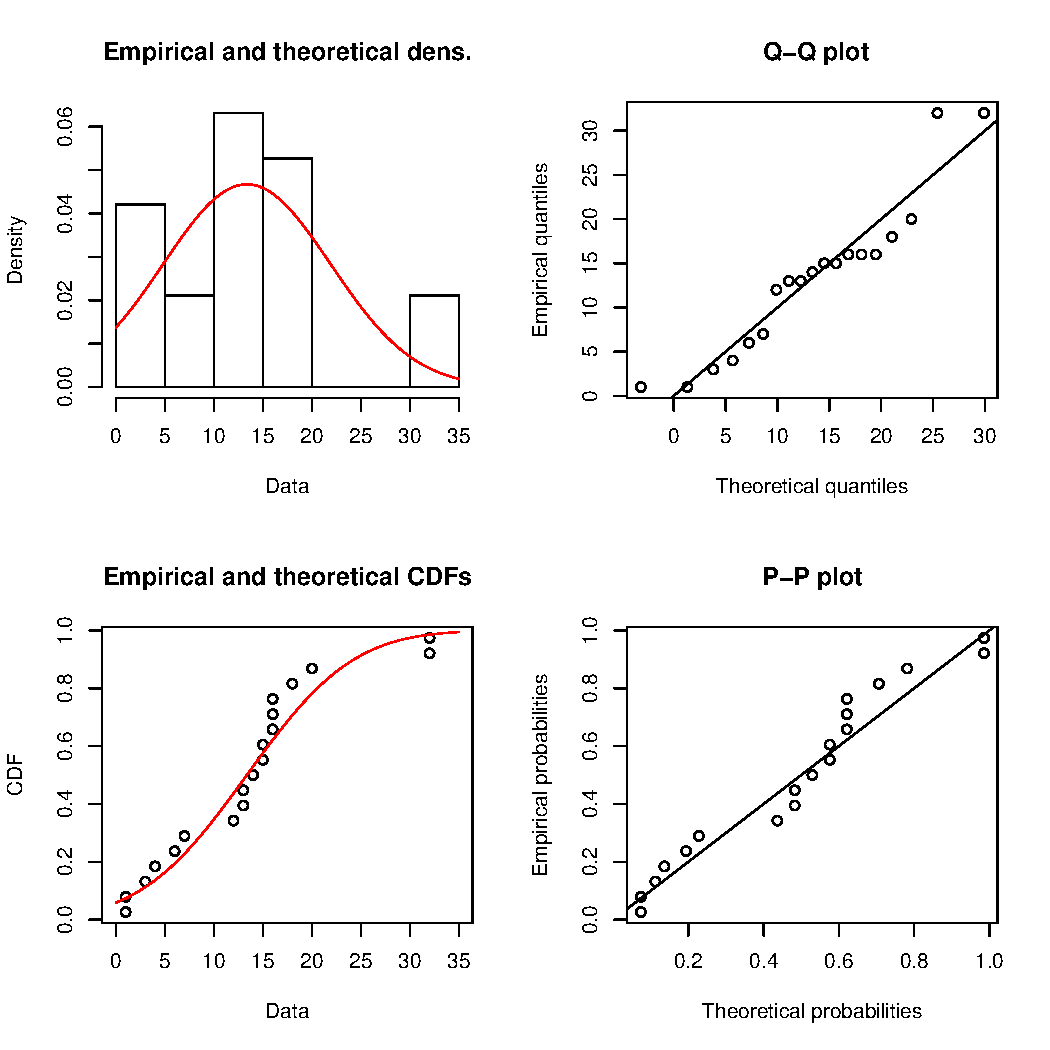
\includegraphics[width=\maxwidth]{figure/unnamed-chunk-5-1} 

\end{knitrout}

\begin{knitrout}
\definecolor{shadecolor}{rgb}{0.969, 0.969, 0.969}\color{fgcolor}\begin{kframe}
\begin{alltt}
\hlstd{fit.gamma}\hlopt{$}\hlstd{estimate} \hlcom{#alpha}
\end{alltt}
\begin{verbatim}
##     shape      rate 
## 1.6708800 0.1249822
\end{verbatim}
\begin{alltt}
\hlstd{fit.gamma}\hlopt{$}\hlstd{sd} \hlcom{#beta}
\end{alltt}
\begin{verbatim}
##      shape       rate 
## 0.49735268 0.04330907
\end{verbatim}
\begin{alltt}
\hlkwd{plot}\hlstd{(fit.gamma)}
\end{alltt}
\end{kframe}
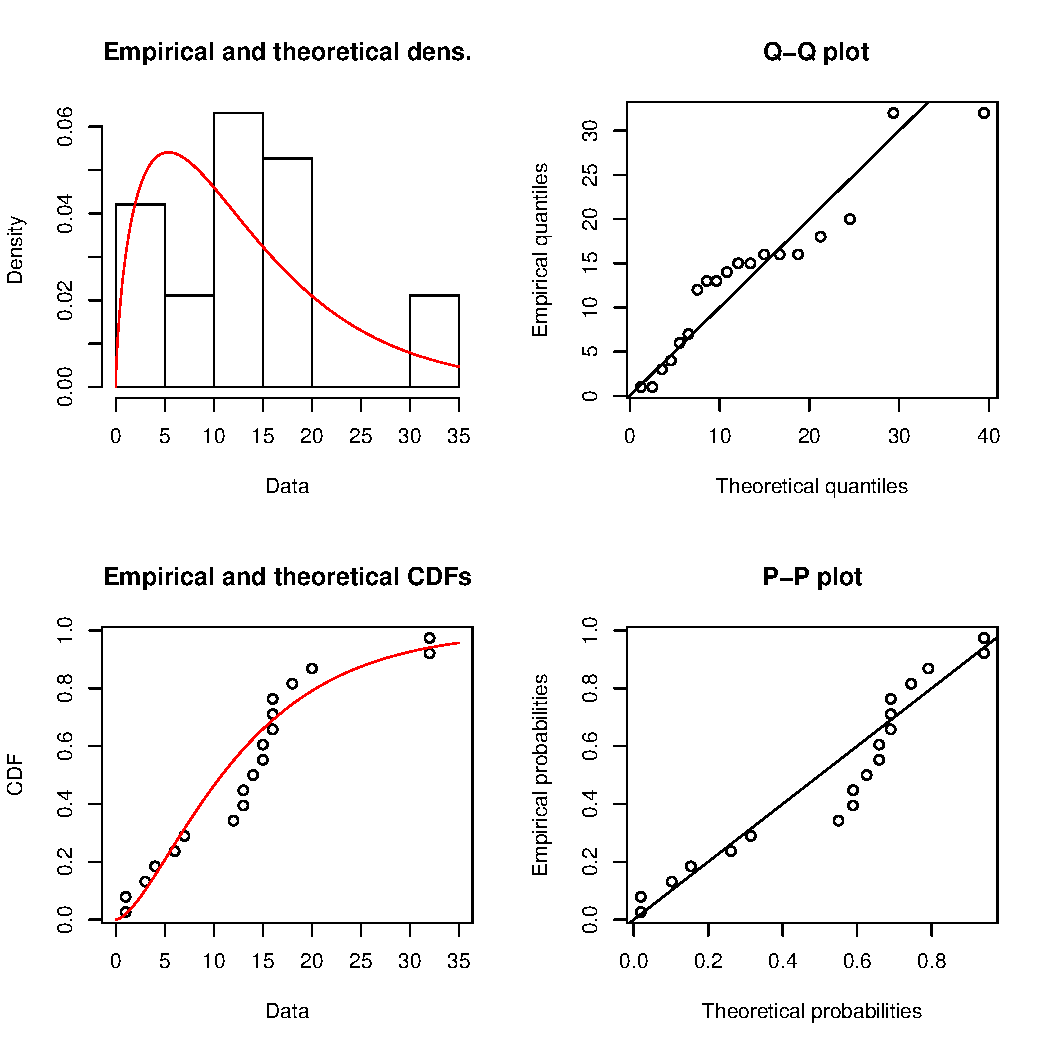
\includegraphics[width=\maxwidth]{figure/unnamed-chunk-6-1} 

\end{knitrout}

\begin{knitrout}
\definecolor{shadecolor}{rgb}{0.969, 0.969, 0.969}\color{fgcolor}\begin{kframe}
\begin{alltt}
\hlstd{fit.lognormal}\hlopt{$}\hlstd{estimate} \hlcom{#mu}
\end{alltt}
\begin{verbatim}
##   meanlog     sdlog 
## 2.2646253 0.9749802
\end{verbatim}
\begin{alltt}
\hlstd{fit.lognormal}\hlopt{$}\hlstd{sd} \hlcom{#sigma}
\end{alltt}
\begin{verbatim}
##   meanlog     sdlog 
## 0.2236758 0.1581619
\end{verbatim}
\begin{alltt}
\hlkwd{plot}\hlstd{(fit.lognormal)}
\end{alltt}
\end{kframe}
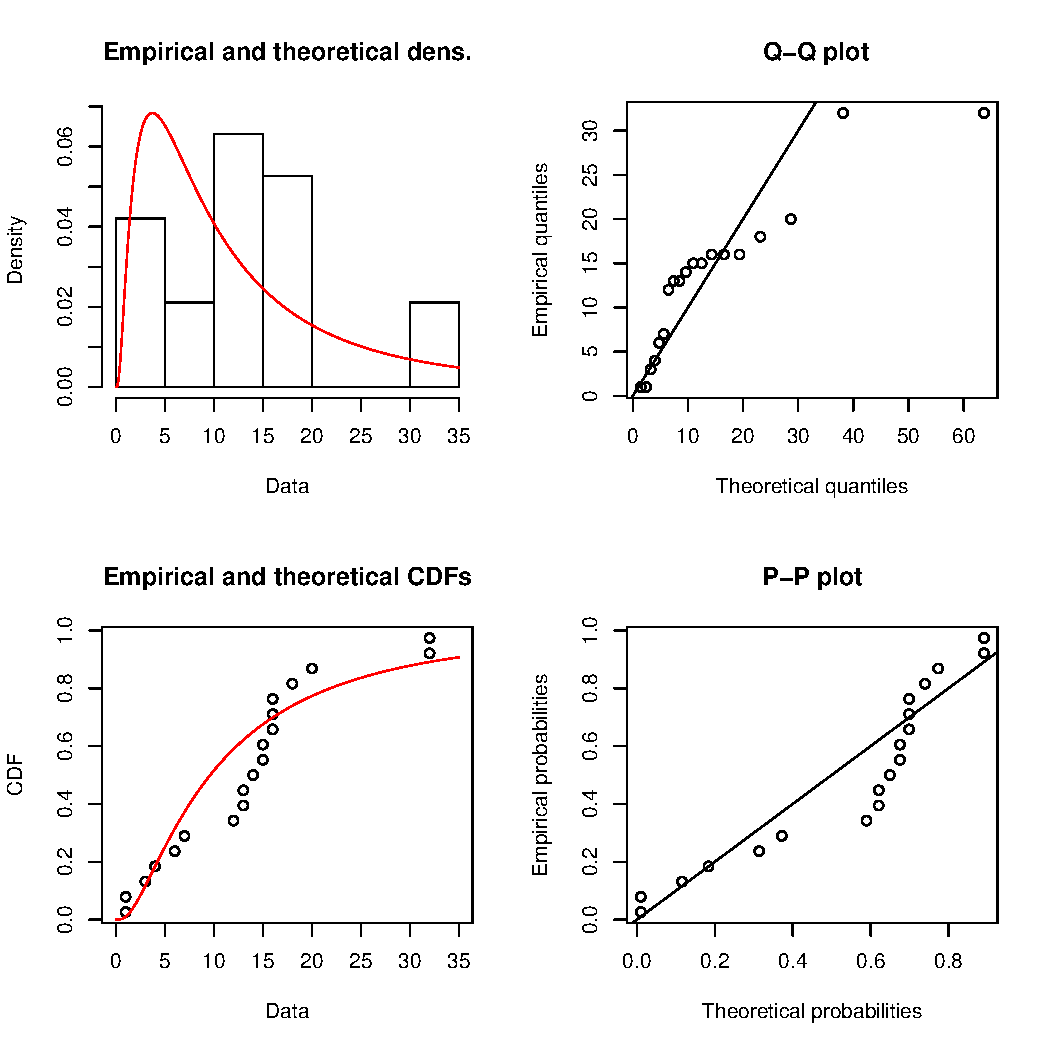
\includegraphics[width=\maxwidth]{figure/unnamed-chunk-7-1} 

\end{knitrout}

En observant les graphes Q-Q plot, on peut déduire que la loi Normale est la loi qui semble le mieux représenter la fonction de densité empirique. 

On en conclut que, la distribution des \emph{Jacob} sur le territoire Lavallois suit une loi Normale avec paramètre $\mu = 13.368421, \sigma = 1.958306$.

\subsection{Maria}
Le persona de Maria possède les caractéristiques suivantes : 
\begin{itemize}
\item 35 ans;
\item\numprint{51000} \$;
\item Comptable.
\end{itemize}
La fonction de prédiction correspond à
\begin{align*}
f_{\mathbb{X}}(x) &= f_{X_{\text{Occupation}}}(\text{Professionnel}) \times f_{X_{\text{Âge}}}(\text{32-39}) \times f_{X_{\text{salaire}}}(\text{\numprint{50000} - \numprint{60000}})
\end{align*}

Ce qui nous permet de trouver le tableau de valeur suivant :
\begin{knitrout}
\definecolor{shadecolor}{rgb}{0.969, 0.969, 0.969}\color{fgcolor}\begin{kframe}
\begin{verbatim}
## # A tibble: 19 x 5
##       X1 Prediction `Pop femme 32_39` `Pop service` Salaire
##    <chr>      <int>             <int>         <dbl>   <int>
##  1   H7A          3              1214    0.01375016    1445
##  2   H7B          0               169    0.01375016     205
##  3   H7C          1               422    0.01375016     470
##  4   H7E          3              1081    0.01375016    1965
##  5   H7G          2              1035    0.01375016    1150
##  6   H7H          2               811    0.01375016    1130
##  7   H7J          0               107    0.01375016     170
##  8   H7K          3              1016    0.01375016    1685
##  9   H7L          6              2053    0.01375016    2875
## 10   H7M          3              1193    0.01375016    1770
## 11   H7N          5              2472    0.01375016    2205
## 12   H7P          5              1793    0.01375016    2395
## 13   H7R          4              1659    0.01375016    2065
## 14   H7S          1               381    0.01375016     385
## 15   H7T          3              1338    0.01375016    1440
## 16   H7V          1              1039    0.01375016     760
## 17   H7W          3              2029    0.01375016    1900
## 18   H7X          3              1362    0.01375016    1755
## 19   H7Y          2               551    0.01375016     725
## [1] 3
\end{verbatim}
\end{kframe}
\end{knitrout}
On remarque que la moyenne correspond à 3 pour l'ensemble du territoire de l'ile de Laval. Autrement dit, il y a en moyenne une femme âgée de 32 et 39 ans qui est comptable et qui fait entre \numprint{50000}\$ et \numprint{60000} \$ par année. Le résultat est cohérent avec les données initiales du recensement. En effet, selon les données de Statistique Canada, il y a en moyenne 1143 femmes âgées de 32 et 39 ans par région de tri d'acheminement. De plus, il n'y a qu'en moyenne 1394 Lavallois par RTA qui ont un salaire annuel dans la même tranche que Maria. Autrement dit, en moyenne 72 femmes âgées de 32 et 39 ans ont un salaire annuel entre \numprint{50000}\$ et \numprint{60000} \$ par année. N'ayant pas réussi à trouver des données segmentez par type de profession aussi précise que comptable, il a été déduit que la profession de comptable se retrouve dans les catégories suivantes : Gestion, affaires, finance et service. Ce qui a permis de déterminer la proportion de comptables à $3.735033 \%$. On obtient ainsi la distribution illustrée précédemment. \newline

\subsubsection*{Analyse des graphiques de distribution}

On présente les graphiques de l'ajustement des données des régions de tri d'acheminement de Laval sur la loi Normale \footnote{Il a été impossible d'ajuster d'autres lois sur les données.}.


\begin{knitrout}
\definecolor{shadecolor}{rgb}{0.969, 0.969, 0.969}\color{fgcolor}\begin{kframe}
\begin{alltt}
\hlstd{fit.normal}\hlopt{$}\hlstd{estimate} \hlcom{#mu}
\end{alltt}
\begin{verbatim}
##     mean       sd 
## 2.631579 1.596395
\end{verbatim}
\begin{alltt}
\hlstd{fit.normal}\hlopt{$}\hlstd{sd} \hlcom{#sigma}
\end{alltt}
\begin{verbatim}
##      mean        sd 
## 0.3662381 0.2589690
\end{verbatim}
\begin{alltt}
\hlkwd{plot}\hlstd{(fit.normal)}
\end{alltt}
\end{kframe}
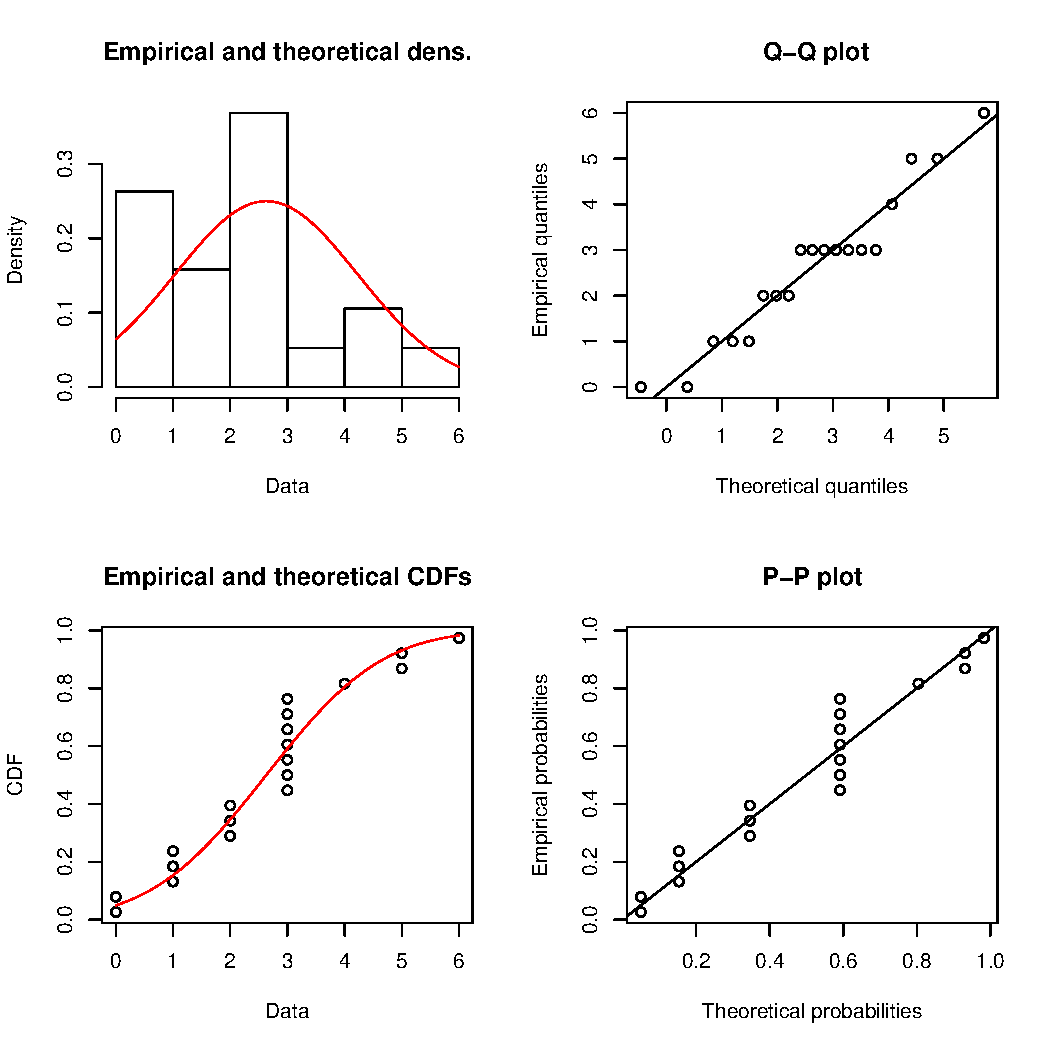
\includegraphics[width=\maxwidth]{figure/unnamed-chunk-10-1} 

\end{knitrout}

En observant les graphes Q-Q plot, on peut déduire que la loi Normale n'est pas une loi appropriée pour représenter la fonction de densité empirique. Il semblerait que la qualité des données sur l'occupation et l'hypothèse de distribution n'est pas adéquate et nécessiterait une amélioration. Une piste de solution est abordée plus loin.

On en conclut que la distribution n'est pas ajustable sur une loi Normale.

\subsection{David}
Le persona de Maria possède les caractéristiques suivantes : 
\begin{itemize}
\item 45 ans;
\item\numprint{105000} \$;
\item PME.
\end{itemize}
La fonction de prédiction correspond à
\begin{align*}
f_{\mathbb{X}}(x) &= f_{X_{\text{Occupation}}}(\text{PME}) \times f_{X_{\text{Âge}}}(\text{40-52}) \times f_{X_{\text{salaire}}}(\text{\numprint{100000} et +})
\end{align*}

Ce qui nous permet de trouver le tableau de valeur suivant :
\begin{knitrout}
\definecolor{shadecolor}{rgb}{0.969, 0.969, 0.969}\color{fgcolor}\begin{kframe}
\begin{verbatim}
## # A tibble: 19 x 5
##       X1 Prediction `Pop homme 40_52`  `Pop PME` Salaire
##    <chr>      <int>             <int>      <dbl>   <int>
##  1   H7A          0              2010 0.04799292      90
##  2   H7B          0               293 0.04799292      20
##  3   H7C          0               962 0.04799292      40
##  4   H7E          1              2471 0.04799292     295
##  5   H7G          0              1678 0.04799292     130
##  6   H7H          0              1392 0.04799292     100
##  7   H7J          0               200 0.04799292      20
##  8   H7K          1              2188 0.04799292     220
##  9   H7L          2              3904 0.04799292     395
## 10   H7M          1              2185 0.04799292     190
## 11   H7N          1              3466 0.04799292     165
## 12   H7P          1              3468 0.04799292     265
## 13   H7R          1              3146 0.04799292     210
## 14   H7S          0               635 0.04799292      30
## 15   H7T          1              2151 0.04799292     180
## 16   H7V          0              1749 0.04799292      45
## 17   H7W          1              3448 0.04799292     210
## 18   H7X          2              2906 0.04799292     310
## 19   H7Y          1              1178 0.04799292     190
## [1] 1
\end{verbatim}
\end{kframe}
\end{knitrout}
On remarque que la moyenne correspond à 1 pour l'ensemble du territoire de l'ile de Laval. Autrement dit, il y a en moyenne un homme âgé de 40 et 52 ans qui est propriétaire d'une PME et qui fait plus de \numprint{100000} \$ par année. Le résultat est cohérent avec les données initiales du recensement. En effet, selon les données de Statistique Canada, il y a en moyenne 2075 hommes âgés de 40 et 52 ans par région de tri d'acheminement. De plus, il n'y a qu'en moyenne 163 Lavallois qui font plus de \numprint{100000} \$ par année. Autrement dit, en moyenne 43 hommes Lavalois possèdent les deux premières caractéristiques. N'ayant pas réussi à trouver des données segmentées par type de profession aussi précise que propriétaire de PME, il a été déduit que cette profession se retrouve dans les catégories suivantes : Gestion,  affaires et finance. Ce qui a permis d'établir que la proportion de propriétaires de PME est de $4.799292 \%$. La distribution prédite est donc cohérente avec les données observées.

\subsubsection*{Analyse des graphiques de distribution}

On présente les graphiques de l'ajustement des données des régions de tri d'acheminement de Laval sur la loi Normale\footnote{Il a été impossible d'ajuster d'autres lois sur les données.}.


\begin{knitrout}
\definecolor{shadecolor}{rgb}{0.969, 0.969, 0.969}\color{fgcolor}\begin{kframe}
\begin{alltt}
\hlstd{fit.normal}\hlopt{$}\hlstd{estimate} \hlcom{#mu}
\end{alltt}
\begin{verbatim}
##      mean        sd 
## 0.6842105 0.6531407
\end{verbatim}
\begin{alltt}
\hlstd{fit.normal}\hlopt{$}\hlstd{sd} \hlcom{#sigma}
\end{alltt}
\begin{verbatim}
##      mean        sd 
## 0.1498408 0.1059523
\end{verbatim}
\begin{alltt}
\hlkwd{plot}\hlstd{(fit.normal)}
\end{alltt}
\end{kframe}
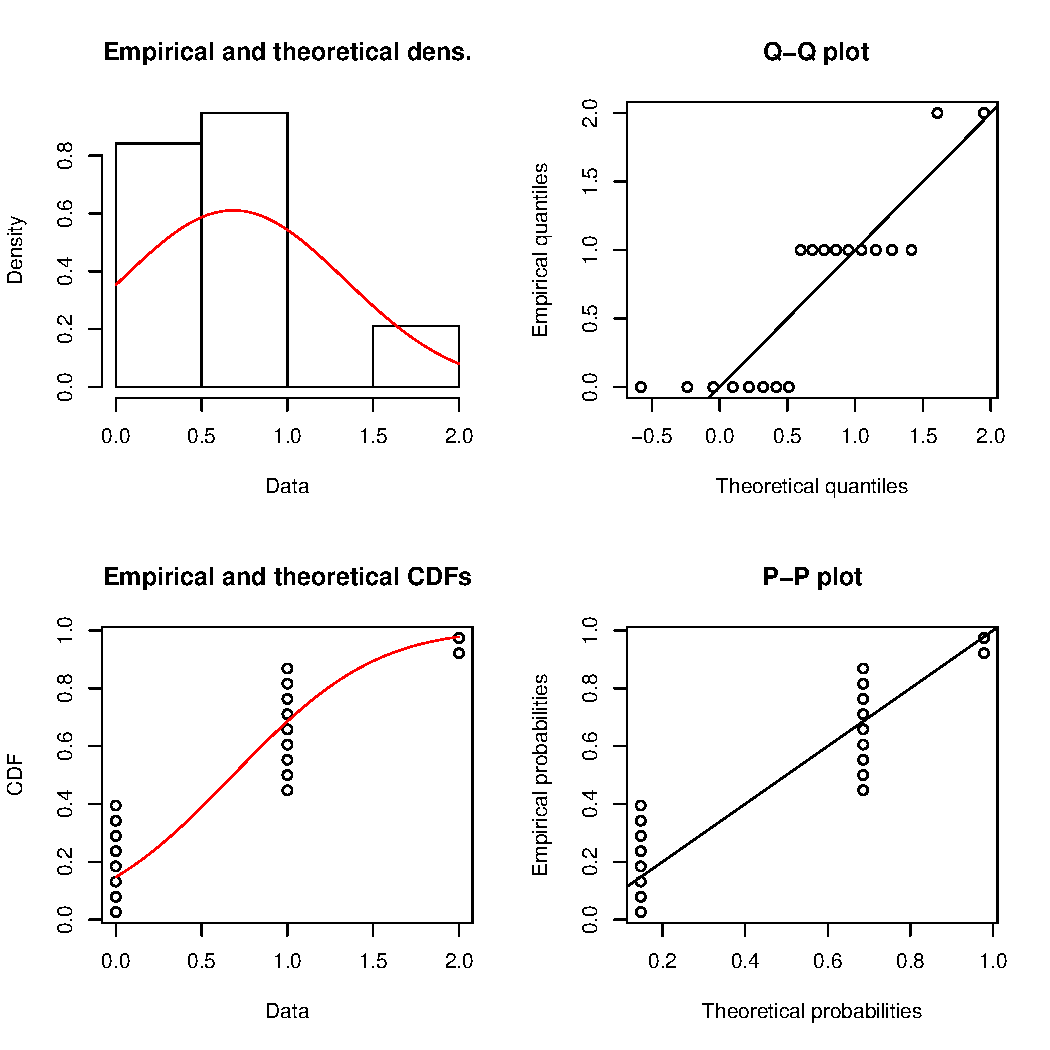
\includegraphics[width=\maxwidth]{figure/unnamed-chunk-13-1} 

\end{knitrout}

En observant les graphes Q-Q plot, on peut déduire que la loi Normale n'est pas une loi approprié pour représenter la fonction de densité empirique. On suppose la même problématique soulevé lors de l'analyse de Maria.

\subsection{Claire}
Le persona de Claire possède les caractéristiques suivantes : 
\begin{itemize}
\item 61 ans;
\item\numprint{50000} \$;
\item enseignante.
\end{itemize}
La fonction de prédiction correspond à
\begin{align*}
f_{\mathbb{X}}(x) &= f_{X_{\text{Occupation}}}(\text{enseignante}) \times f_{X_{\text{Âge}}}(\text{53 - 65}) \times f_{X_{\text{salaire}}}(\text{\numprint{50000} - \numprint{60000}})
\end{align*}

Ce qui nous permet de trouver le tableau de valeur suivant :
\begin{knitrout}
\definecolor{shadecolor}{rgb}{0.969, 0.969, 0.969}\color{fgcolor}\begin{kframe}
\begin{verbatim}
## # A tibble: 19 x 5
##       X1 Prediction `Pop femme 53_65` `Pop enseign` Salaire
##    <chr>      <int>             <int>         <dbl>   <int>
##  1   H7A          1              1854    0.01046631    1445
##  2   H7B          0               283    0.01046631     205
##  3   H7C          0               730    0.01046631     470
##  4   H7E          2              2468    0.01046631    1965
##  5   H7G          1              1888    0.01046631    1150
##  6   H7H          1              1238    0.01046631    1130
##  7   H7J          0               270    0.01046631     170
##  8   H7K          2              2278    0.01046631    1685
##  9   H7L          3              3131    0.01046631    2875
## 10   H7M          2              2991    0.01046631    1770
## 11   H7N          2              3645    0.01046631    2205
## 12   H7P          2              3275    0.01046631    2395
## 13   H7R          2              2583    0.01046631    2065
## 14   H7S          0               611    0.01046631     385
## 15   H7T          1              2185    0.01046631    1440
## 16   H7V          1              1851    0.01046631     760
## 17   H7W          2              3591    0.01046631    1900
## 18   H7X          1              2047    0.01046631    1755
## 19   H7Y          1               771    0.01046631     725
## [1] 1
\end{verbatim}
\end{kframe}
\end{knitrout}
On remarque que la moyenne correspond à 1 pour l'ensemble du territoire de l'ile de Laval. Autrement dit, il y a en moyenne une femme âgée de 53 et 65 ans qui est enseignantes et qui fait entre \numprint{50000}\$ et \numprint{60000} \$  par année. Le résultat est cohérent avec les données initiales du recensement. En effet, selon les données de Statistique Canada, il y a en moyenne 1986 femmes âgées de 53 et 65 ans par région de tri d'acheminement. De plus, il n'y a en moyenne 1394 Lavallois qui font entre  \numprint{50000}\$ et \numprint{60000} \$  par année. Autrement dit, en moyenne 124 femmes lavalloises possèdent les deux premières caractéristiques. De plus, seulement $1.0466$\% des Québécois sont dans l'enseignement. 

\subsubsection*{Analyse des graphiques de distribution}

On présente les graphiques de l'ajustement des données des régions de tri d'acheminement de Laval sur la loi Normale\footnote{Il a été impossible d'ajuster d'autres lois sur les données.}.

\begin{knitrout}
\definecolor{shadecolor}{rgb}{0.969, 0.969, 0.969}\color{fgcolor}\begin{kframe}
\begin{alltt}
\hlstd{fit.normal}\hlopt{$}\hlstd{estimate} \hlcom{#mu}
\end{alltt}
\begin{verbatim}
##      mean        sd 
## 1.2631579 0.8486587
\end{verbatim}
\begin{alltt}
\hlstd{fit.normal}\hlopt{$}\hlstd{sd} \hlcom{#sigma}
\end{alltt}
\begin{verbatim}
##      mean        sd 
## 0.1946957 0.1376698
\end{verbatim}
\begin{alltt}
\hlkwd{plot}\hlstd{(fit.normal)}
\end{alltt}
\end{kframe}
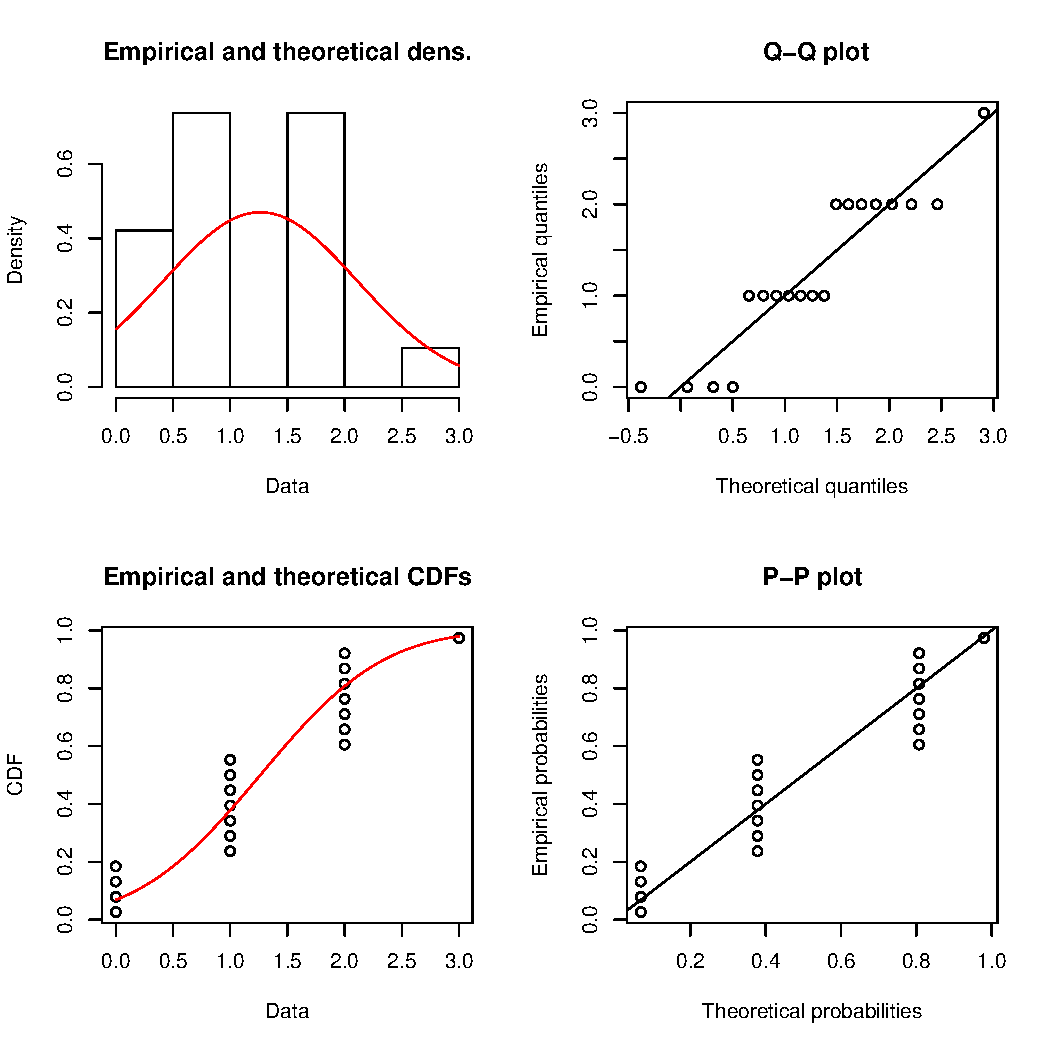
\includegraphics[width=\maxwidth]{figure/unnamed-chunk-16-1} 

\end{knitrout}

En observant les graphes Q-Q plot, on peut déduire que la loi Normale n'est pas une loi approprié pour représenter la fonction de densité empirique. On suppose la même problématique soulevé lors de l'analyse de Maria.

\subsection{Daniel}
Le persona de Daniel possède les caractéristiques suivantes : 
\begin{itemize}
\item 71 ans;
\item\numprint{43000} \$;
\item retraité.
\end{itemize}
La fonction de prédiction correspond à
\begin{align*}
f_{\mathbb{X}}(x) &= f_{X_{\text{Occupation}}}(\text{retraité}) \times f_{X_{\text{Âge}}}(\text{66 - 76}) \times f_{X_{\text{salaire}}}(\text{\numprint{40000} - \numprint{50000}})
\end{align*}

Ce qui nous permet de trouver le tableau de valeur suivant :
\begin{knitrout}
\definecolor{shadecolor}{rgb}{0.969, 0.969, 0.969}\color{fgcolor}\begin{kframe}
\begin{verbatim}
## # A tibble: 19 x 5
##       X1 Prediction `Pop homme 66_76` `Pop retraite` Salaire
##    <chr>      <int>             <int>          <dbl>   <int>
##  1   H7A         84               757   1.225865e-07    2325
##  2   H7B         16               131   1.225865e-07     380
##  3   H7C         39               426   1.225865e-07     830
##  4   H7E        129              1292   1.225865e-07    2640
##  5   H7G         87               975   1.225865e-07    1895
##  6   H7H         52               449   1.225865e-07    1590
##  7   H7J         13               128   1.225865e-07     225
##  8   H7K         85               833   1.225865e-07    2260
##  9   H7L        108              1094   1.225865e-07    3685
## 10   H7M        140              1434   1.225865e-07    2715
## 11   H7N        159              1725   1.225865e-07    3900
## 12   H7P        164              1577   1.225865e-07    3640
## 13   H7R        116              1124   1.225865e-07    3095
## 14   H7S         29               315   1.225865e-07     665
## 15   H7T        105              1121   1.225865e-07    2255
## 16   H7V         71              1081   1.225865e-07    1485
## 17   H7W        188              2363   1.225865e-07    3305
## 18   H7X         81               923   1.225865e-07    2285
## 19   H7Y         23               245   1.225865e-07     905
## [1] 89
\end{verbatim}
\end{kframe}
\end{knitrout}
On remarque que la moyenne correspond à 89 pour l'ensemble du territoire de l'ile de Laval. Autrement dit, il y a en moyenne 89 hommes âgés de 66 et 76 ans qui sont à la retraite et qui font entre \numprint{40000}\$ et \numprint{50000} \$  par année. Le résultat est cohérent avec les données initiales du recensement. En effet, selon les données de Statistique Canada, il y a en moyenne 947 hommes âgés de 66 et 76 ans par région de tri d'acheminement. De plus, il n'y a en moyenne 2109 Lavallois qui font entre  \numprint{40000}\$ et \numprint{50000} \$  par année. Autrement dit, en moyenne 89 hommes lavallois possèdent les deux premières caractéristiques. Ce qui est cohérent, car il a été supposé que toutes personnes de plus 65 ans est automatiquement à la retraite. De plus, on rappelle qu'avec la retraite de la génération \emph{baby-boomer} une grande portion de la population est à la retraite.

\subsubsection*{Analyse des graphiques de distribution}

On présente les graphiques de l'ajustement des données des régions de tri d'acheminement de Laval sur les trois lois suivantes, Normale, Gamma et LogNormale.

\begin{knitrout}
\definecolor{shadecolor}{rgb}{0.969, 0.969, 0.969}\color{fgcolor}\begin{kframe}
\begin{alltt}
\hlstd{fit.normal}\hlopt{$}\hlstd{estimate} \hlcom{#mu}
\end{alltt}
\begin{verbatim}
##     mean       sd 
## 88.89474 50.90538
\end{verbatim}
\begin{alltt}
\hlstd{fit.normal}\hlopt{$}\hlstd{sd} \hlcom{#sigma}
\end{alltt}
\begin{verbatim}
##      mean        sd 
## 11.678494  8.257943
\end{verbatim}
\begin{alltt}
\hlkwd{plot}\hlstd{(fit.normal)}
\end{alltt}
\end{kframe}
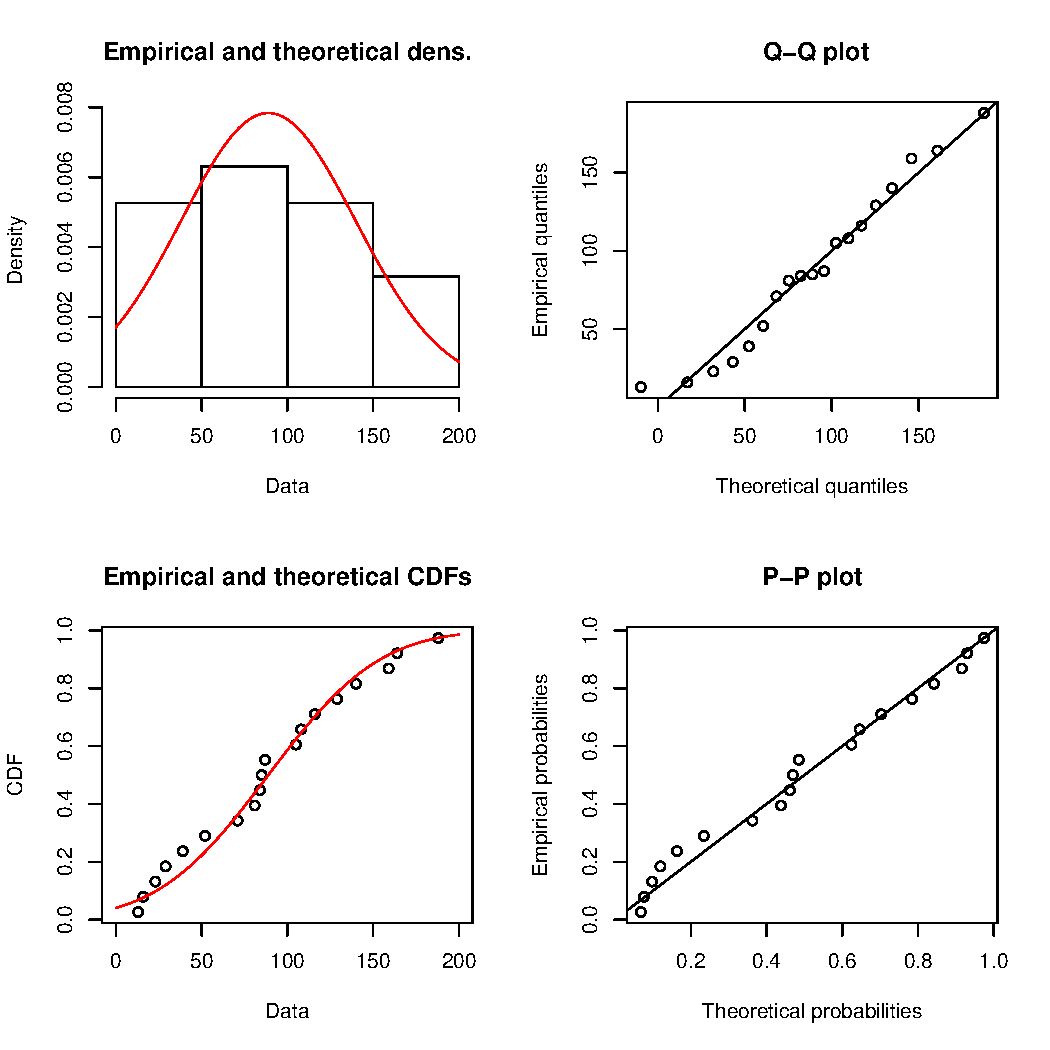
\includegraphics[width=\maxwidth]{figure/unnamed-chunk-19-1} 

\end{knitrout}

\begin{knitrout}
\definecolor{shadecolor}{rgb}{0.969, 0.969, 0.969}\color{fgcolor}\begin{kframe}
\begin{alltt}
\hlstd{fit.gamma}\hlopt{$}\hlstd{estimate} \hlcom{#alpha}
\end{alltt}
\begin{verbatim}
##      shape       rate 
## 2.25687826 0.02538995
\end{verbatim}
\begin{alltt}
\hlstd{fit.gamma}\hlopt{$}\hlstd{sd} \hlcom{#beta}
\end{alltt}
\begin{verbatim}
##       shape        rate 
## 0.682239619 0.008578526
\end{verbatim}
\begin{alltt}
\hlkwd{plot}\hlstd{(fit.gamma)}
\end{alltt}
\end{kframe}
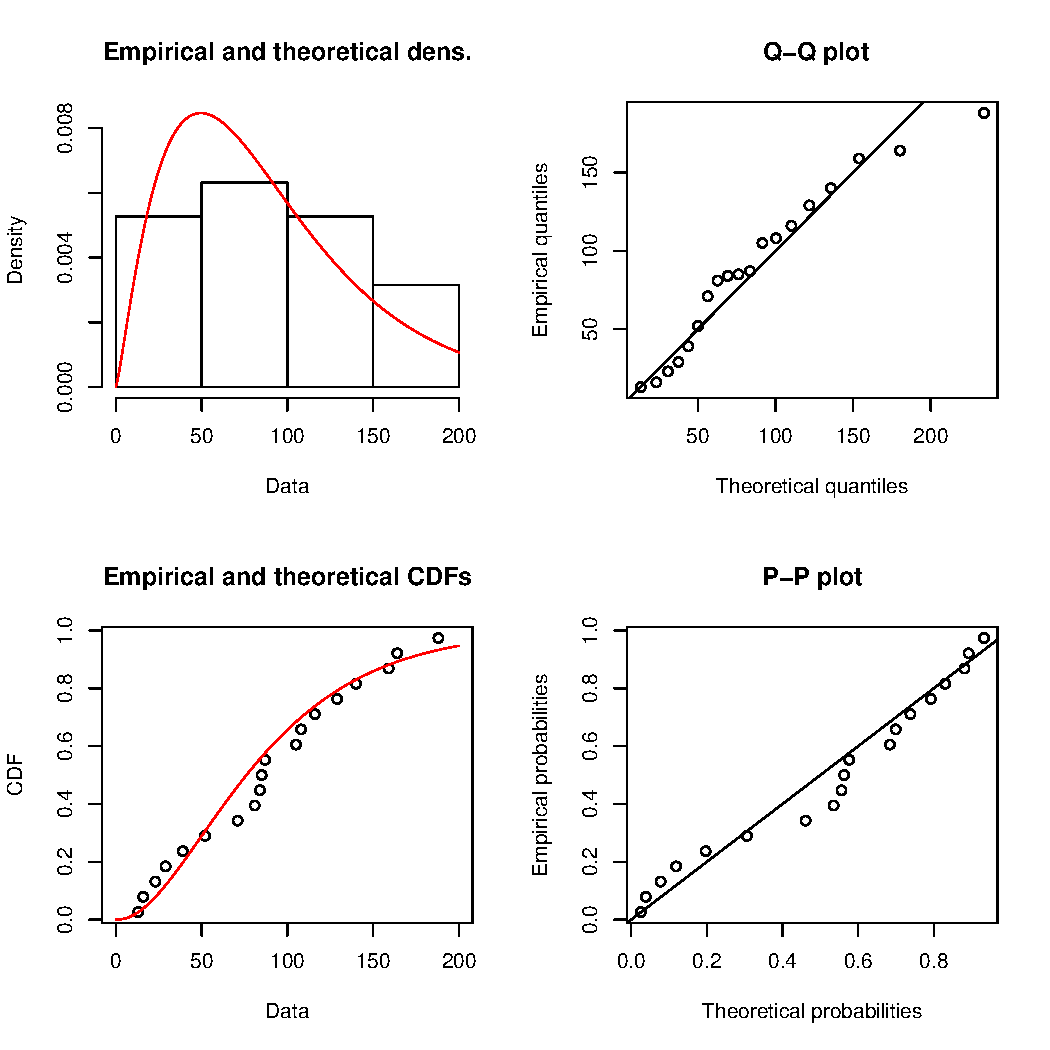
\includegraphics[width=\maxwidth]{figure/unnamed-chunk-20-1} 

\end{knitrout}

\begin{knitrout}
\definecolor{shadecolor}{rgb}{0.969, 0.969, 0.969}\color{fgcolor}\begin{kframe}
\begin{alltt}
\hlstd{fit.lognormal}\hlopt{$}\hlstd{estimate} \hlcom{#mu}
\end{alltt}
\begin{verbatim}
##   meanlog     sdlog 
## 4.2498941 0.7757426
\end{verbatim}
\begin{alltt}
\hlstd{fit.lognormal}\hlopt{$}\hlstd{sd} \hlcom{#sigma}
\end{alltt}
\begin{verbatim}
##   meanlog     sdlog 
## 0.1779676 0.1258411
\end{verbatim}
\begin{alltt}
\hlkwd{plot}\hlstd{(fit.lognormal)}
\end{alltt}
\end{kframe}
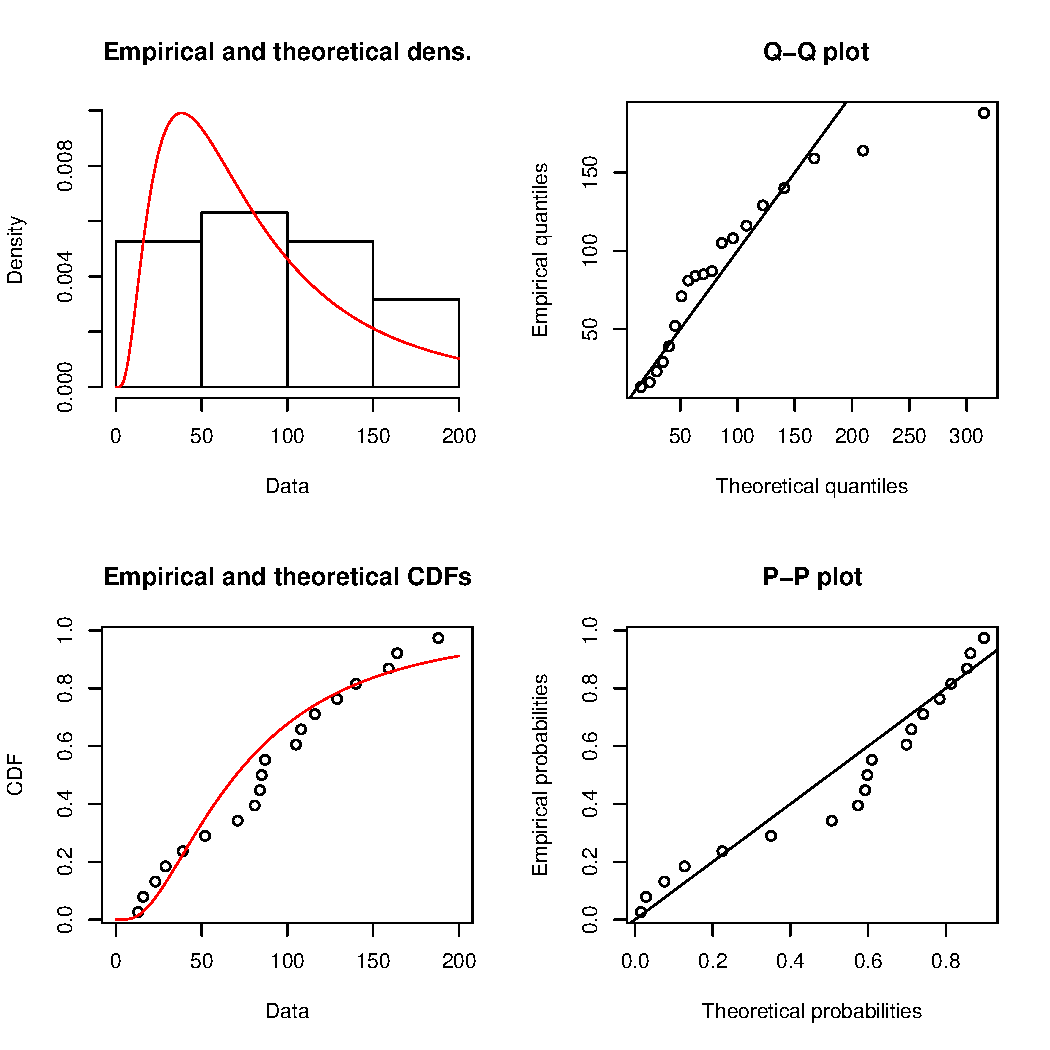
\includegraphics[width=\maxwidth]{figure/unnamed-chunk-21-1} 

\end{knitrout}

En observant les graphes Q-Q plot, on peut déduire que la loi Normale est la loi qui semble le mieux représenter la fonction de densité empirique. \newline

On en conclut que, la distribution des \emph{Daniel} sur le territoire Lavallois suis une loi Normale avec paramètre $\mu = 88.89474, \sigma = 11.678494$.

\subsection*{Conclusion}
Pour conclure, après l'analyse des différentes variables et l'analyse de la distribution des personas, on constate que les différentes hypothèses utilisées dans le modèle sont cohérentes. De plus, il devient ainsi possible de bien représenter la distribution des différents personas.


\section{Pistes d'améliorations}

Lors de la présentation des hypothèses retenues, la problématique sur la distribution des étudiants dans les RTA a été soulevée. En effet, si l'on désire améliorer la fiabilité de la prédiction de cette variable, il serait intéressant de créer un modèle plus complexe pour cette variable. En utilisant les données de fréquentations des établissements, de la méthode de transport ainsi que l'établissement d'un zonage en périphérie des établissements. Ce zonage correspondant à la probabilité de retrouver un étudiant dans cette zone. Il serait alors possible d'établir l'étalement urbain des étudiants. Par la suite, en superposant les RTA sur le zonage d'étalement, il serait plus facile d'établir avec précision la distribution des étudiants par RTA. 
\newline

Une seconde piste d'amélioration serait d'améliorer l'hypothèse d'âge à la retraite. Tel que discuté plus tôt, le facteur temps ayant empêché l'approfondissement de cette variable, il serait pertinent de corriger cette solution. En effet, de nombreuses données complètes existent sur la retraite. Il aurait été possible de déterminer la distribution de l'âge à la retraite et de déterminer, conjointement avec le recensement, la distribution de la retraite anticipée, de la retraite progressive et de la retraite tardive. Ainsi, la qualité de la prédiction de cette variable serait grandement améliorée.
\newline

Une troisième piste d'amélioration a été observée lors de l'analyse des résultats, l'hypothèse initiale de distribution uniforme des occupations ne semble pas être adéquate, on remarque pour la plupart des personas, cette hypothèse fait perdre beaucoup de précision au modèle. De plus, la faible segmentation des données nuit aussi grandement à la capacité du modèle de capter l'information réelle. La recherche de donnée plus complète serait à considérer pour améliorer l'efficacité du modèle.
\newline

Une dernière piste d'amélioration du modèle concerne l'ajout de variables, soit l'ajout d'une variable de canaux de communication favoris et de la variable méthode de transport. Cet ajout permettrait d'améliorer le produit offert aux agences. En effet, il serait pertinent de modéliser le canal de communication favori des personas, soit numérique, téléphonique et postal. Ainsi, les agences seraient en mesure de mieux cibler la méthode pour contacter les clients potentiels. De plus, la variable de méthode de transport permet d'ajouter la distribution des personas utilisant un véhicule automobile pour se rendre quotidiennement au lieu de travail. Cette variable permettrait de mieux cibler l'offre de produit aux clients potentiels en plus de mieux cibler les offres de rabais de type assurance automobile et habitation.
\newline

Pour conclure, en appliquant les pistes de solutions, la qualité de prédiction du modèle serait grandement améliorée ainsi que la qualité du service offert aux agences. C'est pourquoi je recommande que l'approfondissement du projet soit considéré pour améliorer la qualité métrique d'estimation et la qualité d'affaire du projet.
\newline

\section{Conclusion}

Pour conclure, le modèle présenter dans ce projet permet de modéliser de nombreuses variables différentes ainsi que la distribution des personas. La modélisation et la distribution des variables peuvent être jointes ou individuelles. La possibilité de visualiser cette distribution sur une carte est possible via l'application jointe avec le projet. Le modèle présente différents avantages, tels que la simplification et la portabilité du modèle. Par contre, on a bien démontré que certaines hypothèses et données ne semblent pas concluantes pour prédire la distribution des occupations des personas. La principale faiblesse du modèle réside dans cette variable. Malgré tout, le modèle semble concluant dans la représentation de la distribution des personas.


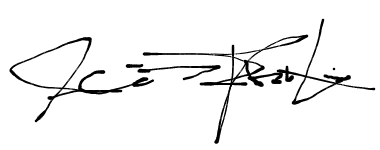
\includegraphics[height=3cm, width = 4cm]{fig/signature.png}

\end{document}
